% !TEX TS-program = pdflatex
% !TEX encoding = UTF-8 Unicode

% This is a simple template for a LaTeX document using the "article" class.
% See "book", "report", "letter" for other types of document.

\documentclass[11pt]{article} % use larger type; default would be 10pt

\usepackage[utf8]{inputenc} % set input encoding (not needed with XeLaTeX)

%%% Examples of Article customizations
% These packages are optional, depending whether you want the features they provide.
% See the LaTeX Companion or other references for full information.

%%% PAGE DIMENSIONS
\usepackage{geometry} % to change the page dimensions
\geometry{a4paper} % or letterpaper (US) or a5paper or....
% \geometry{margin=2in} % for example, change the margins to 2 inches all round
% \geometry{landscape} % set up the page for landscape
%   read geometry.pdf for detailed page layout information

\usepackage{graphicx} % support the \includegraphics command and options

% \usepackage[parfill]{parskip} % Activate to begin paragraphs with an empty line rather than an indent

%%% PACKAGES
\usepackage{booktabs} % for much better looking tables
\usepackage{array} % for better arrays (eg matrices) in maths
\usepackage{paralist} % very flexible & customisable lists (eg. enumerate/itemize, etc.)
\usepackage{verbatim} % adds environment for commenting out blocks of text & for better verbatim
\usepackage{subfig} % make it possible to include more than one captioned figure/table in a single float
% These packages are all incorporated in the memoir class to one degree or another...

\usepackage{url}

%%% HEADERS & FOOTERS
\usepackage{fancyhdr} % This should be set AFTER setting up the page geometry
\pagestyle{fancy} % options: empty , plain , fancy
\renewcommand{\headrulewidth}{0pt} % customise the layout...
\lhead{}\chead{}\rhead{}
\lfoot{}\cfoot{\thepage}\rfoot{}

%%% SECTION TITLE APPEARANCE
\usepackage{sectsty}
\allsectionsfont{\sffamily\mdseries\upshape} % (See the fntguide.pdf for font help)
% (This matches ConTeXt defaults)

%%% ToC (table of contents) APPEARANCE
\usepackage[nottoc,notlof,notlot]{tocbibind} % Put the bibliography in the ToC
\usepackage[titles,subfigure]{tocloft} % Alter the style of the Table of Contents
\renewcommand{\cftsecfont}{\rmfamily\mdseries\upshape}
\renewcommand{\cftsecpagefont}{\rmfamily\mdseries\upshape} % No bold!


\newcommand{\code}{\texttt}

%%% END Article customizations

%%% The "real" document content comes below...

\title{I-EPOS Manual}
\author{Peter Pilgerstorfer}
%\date{} % Activate to display a given date or no date (if empty),
         % otherwise the current date is printed 

\begin{document}
\maketitle

\section{Introduction}
This documents describes the software that simulates I-EPOS, an algorithm for decentralized combinatorial optimization.

\subsection{Installation and setup}
\begin{itemize}
	\item Download the project repository from \url{https://github.com/epournaras/EPOS}.
	\item Make sure that a version of Oracle Java 8 is installed. You can download it from \url{http://www.oracle.com/technetwork/java/javase/downloads/index.html}.
	\item This should be sufficient to execute I-EPOS.
\end{itemize}
\subsubsection*{Netbeans setup}
Since I-EPOS was developed in the Netbeans IDE, Netbeans can be used to quickly get started in I-EPOS development.
\begin{itemize}
	\item Make sure that Netbeans is installed. You can download it from \url{http://netbeans.org/downloads/}.
	\item Open the EPOS project folder in Netbeans.
	\item Add all libraries from the lib folder to the project.
\end{itemize}

\subsection{Execute the sample simulation}
\begin{itemize}
	\item Start the program
	\begin{itemize}
	\item Run from command line:\\
Navigate to the project directory and execute \code{java -jar EPOS.jar}.
	\item Compile and run in Netbeans:\\
Build and run the project with main class \code{experiment.ui.controller.MainApplication} (default setting).
	\end{itemize}
	\item The configuration window opens as shown in Figure \ref{fig:config}. Run the simulation by clicking the "Run" button.
\begin{figure}[h]
\centering
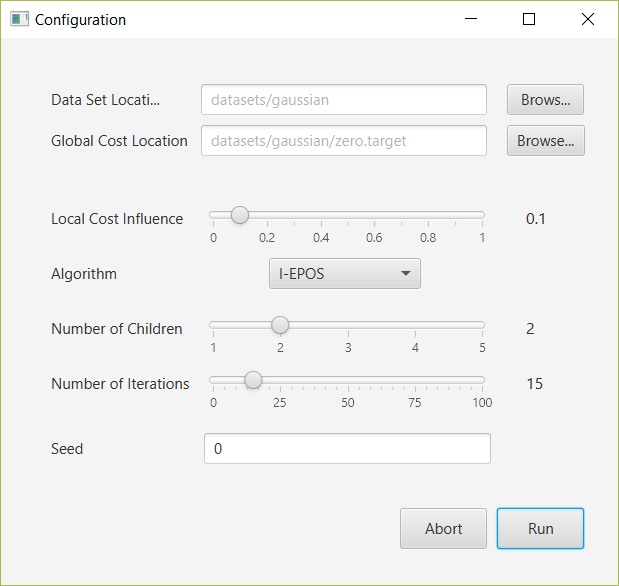
\includegraphics[scale=0.6]{img/configuration.png}
\caption{Simulation configuration}
\label{fig:config}
\end{figure}
	\item The result window opens and shows details about the simulation as shown in Figure \ref{fig:result}. The plot "Global and average local cost" shows the global and local cost in each iteration. The two plots on the bottom show the system state after each iteration. Switch between iterations with the "Next" and "Previous" buttons. The plot "Global Response" shows what the global response, the output of the system, looks like. The plot "Network" shows which agents in the network changed their selections compared to the previous iteration.
\begin{figure}[h]
\centering
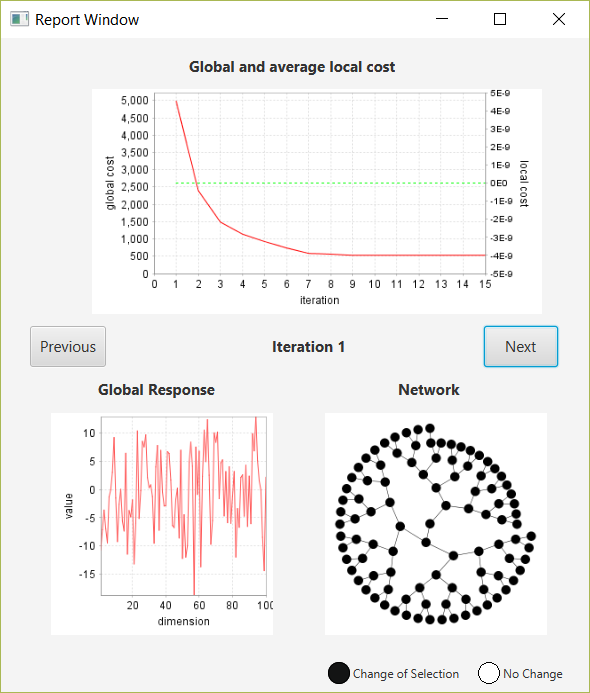
\includegraphics[scale=0.6]{img/results.png}
\caption{Simulation results}
\label{fig:result}
\end{figure}
\end{itemize}

\newpage
\section{Main software components}
The software uses the Protopeer framework to simulate agents in a network. The tree is constructed via the TreeGateway package. The agent logic is dependent on the algorithm in use. For I-EPOS, agents are of type \code{IeposAgent}. For COHDA, agents are of type \code{CohdaAgent}.

When performing a simulations, all agents are started by Protopeer and TreeGateway constructs the tree. After the tree is built, the agents start to execute the algorithm. Each agent logs different metrics that are specified in the configuration. After the algorithm is finished, all logs are gathered and the aggregated results are presented to the user.

\newpage
\section{Use cases}
\subsection{Configure the simulation}
A simulation example is provided in class \code{SimpleExperiment}. It contains a main function that specifies all parameters, starts the simulation and presents the results.

\subsubsection*{Dataset}
The \code{Dataset} interface provides a way to get plans for a given agent via \code{Dataset.getPlans(int agentIdx)}.
There are two classes of datasets implemented:
\begin{itemize}
	\item \code{FileVectorDataset} is a dataset that is read from disk. Only the dataset folder has to be specified. The example datasets are located in the directory 'input-data'. Section \ref{sec:new_dataset} describes the input format for this kind of dataset.
	\item \code{GaussianDataset} is a generated dataset where every plan is a vector drawn from a gaussian distribution. The parameters specify the number and dimensionality of the plans as well as mean and standard deviation of the distribution.
\end{itemize}
The number of agents can be set arbitrarily. However, when using a \code{FileVectorDataset}, the number of agents has to be below \code{FileVectorDataset.getNumAgents()}.

For example a dataset of 100 agents taken from the 'bicycle' dataset can be specified as follows:
\begin{verbatim}
Dataset dataset = new FileVectorDataset("input-data/bicycle");
int numAgents = 100;
\end{verbatim}

\subsubsection*{Cost functions}
The global cost function describes the objective that should be achieved. The local cost function describes what each agent wants to minimize locally. \code{lambda} is the tradeoff between global and local minimization. \code{lambda = 0} means only global cost is minimized, \code{lambda = 1} means only local cost is minimized.
For global cost functions we can choose any implementation of the interface \code{CostFunction} in general. However, for gradient descent based algorithms an instance of \code{DifferentiableCostFunction} is required. A list of possible global cost functions is as follows:
\begin{itemize}
	\item \code{DotCostFunction} minimizes the dot product of a given vector with the global response. See Section \ref{sec:read_vec} how to read the vector from a file. Be aware that the dimensionality of the vector has to match the dimensionality of the dataset.
An example use case for this cost function is minimizing monetary cost. The agent plans contain the amount of resources they consume, and the vector passed to \code{DotCostFunction} describes the price for each resource.
As this is a linear cost function, I-EPOS always finds the optimal value in the first iteration.
	\item \code{SqrDistCostFunction} minimizes the (squared) distance of the global response to a given vector. See Section \ref{sec:read_vec} how to read a vector from a file. Be aware that the dimensionality of the vector has to match the dimensionality of the dataset.
This cost function tries to make the global response as similar to the provided target vector as possible.
	\item \code{VarCostFunction} minimizes the variance of the global response. The effect is that the global response gets stabilized.
	\item \code{StdDevCostFunction} minimizes the standard deviation of the global response. For I-EPOS there is no difference between minimizing standard deviation and minimizing variance, as the functions share the same minima.
	\item \code{MaxCostFunction} (non-differentiable) minimizes the maximum value of the global response. This function is useful to remove peaks in the global response.
\end{itemize}
Local cost functions have to implement the \code{PlanCostFunction} interface. Two functions are implemented:
\begin{itemize}
	\item \code{IndexCostFunction} lets agents select plans with a small index. Therefore the plans in a dataset should be ordered in a way that lists preferable plans first.
	\item \code{PlanScoreCostFunction} lets agents select plans with a small score. The dataset specifies the score for each plan. See Section \ref{sec:new_dataset} for details how to specify this information in a dataset.
\end{itemize}

\noindent For example the variance of the global response can be minimized with the following settings:
\begin{verbatim}
CostFunction globalCostFunc = new VarCostFunction();
LocalCostFunction localCostFunc = null;
double lambda = 0;
\end{verbatim}

\subsubsection*{Network}
The network is considered to be a balanced tree with the same number of children for each inner node. The number of children for inner nodes can be specified.
Note that the binary tree is built before the algorithm execution and it remains static for the duration of the algorithm. Every agent remains at the same position in the tree.

For example a binary tree can be specified as follows:
\begin{verbatim}
int numChildren = 2;
\end{verbatim}

\subsubsection*{Logging}
Next we specify what information we want to gather from the simulation. For this task we specify a \code{LoggingProvider<A>}, where \code{A} is the class of the agent that is used in the simulation.
We then specify all information we want to log by adding \code{AgentLoggingProvider}s. Each \code{AgentLoggingProvider} is responsible for reading and presenting one specific type of data. The output is presented after the simulation by calling the method \\\code{LoggingProvider.print()}. The following loggers are ready to use:
\begin{itemize}
	\item \code{GlobalCostLogger} logs the global cost in each iteration and prints the global cost for each individual iteration averaged over multiple simulations. Note that the sample shown in \code{SimpleExperiment} only performs one simulation. Multiple simulations can be performed with e.g. different seeds for the agents or different datasets. The only requirement is that the same \code{LoggingProvider} is used, so all data is gathered in one place.
	\item \code{LocalCostLogger} logs the average local cost in each iteration and prints the average local cost for each individual iteration averaged over multiple simulations.
	\item \code{TerminationLogger} logs how many iterations it took for the algorithm to terminate. The algorithm is considered terminated if nothing changes between two consecutive iterations.
	\item \code{ProgressLogger} prints symbols every few iterations in order to show how far the algorithm has proceeded. It is only useful for large simulations.
	\item \code{CostViewer} shows a plot with global and (optionally) local cost values for each iteration in a new window. The logger requires \code{GlobalCostLogger} to be added to the \code{LoggingProvider} as well. If the \code{LocalCostLogger} is present, the local cost is also shown in the plot.
	\item \code{GraphLogger} shows a graph of the network at a given iteration in a new window. With the arrow keys you can switch between different iterations. Each agent is represented in a certain color. The color code depends on the specified type \code{GraphLogger.Type}. The following types are available:
	\begin{itemize}
		\item \code{Change} marks each agent that changed its selection in the previous iteration as black and all agents without change as white.
		\item \code{Index} colors each agent based on the index of the selected plan. Agents that selected the plan with minimal index are colored white and agents that selected the plan with maximal index are colored black.
	\end{itemize}
	\item \code{FileWriter} writes the log to the specified directory once \code{LoggingProvider.print()} is executed.
	\item \code{FileReader} reads the log from the specified directory once \code{LoggingProvider.print()} is executed. This logger can be used to show results from a previous simulation that were stored with \code{FileWriter}. A sample application of \code{FileReader} can be seen in \code{ReplayExperiment}.
\end{itemize}

\noindent For example the global response can be logged and presented in a new windwow as follows:
\begin{verbatim}
LoggingProvider loggingProvider = new LoggingProvider();
loggingProvider.add(new GlobalCostLogger());
loggingProvider.add(new CostViewer());
\end{verbatim}

\subsubsection*{Algorithm}
Finally, the optimization algorithm has to be specified. The algorithm is determined by the type of \code{Agent} that is used.
\begin{itemize}
	\item \code{IeposAgent} has quite a few options that were part of the research. We need to specify the number of iterations the algorithm should perform. For problems with less than 1000 agents the (local) optimum is usually found with less than 20 iterations. In addition we can specify a \code{PlanSelector}. The default is \code{IeposPlanSelector}. As part of the research that was done for I-EPOS, gradient descent motivated plan selectors were also developed. However, in general they have lower performance than the default.
	\item \code{CohdaAgent}\footnote{Our COHDA implemetation has some limitations: First, \code{CohdaAgent} does not support local cost. Therefore \code{LocalCostLogger} cannot be used. Second, the algorithm starts with an incomplete global response that is missing data from some agents. It takes \code{log(numAgents)/log(numChildren)} iterations for the global response to be complete. Third, even though COHDA does not require the network to be a tree, only tree networks can be simulated with this software.} is an algorithm that was used as a baseline for performance comparison. We only need to specify the number of iterations for this algorithm.
\end{itemize}

\noindent In order to use the I-EPOS algorithm, the system should consist of \code{IeposAgent} nodes. This can be specified via the following function:
\begin{verbatim}
Function<Integer, Agent> createAgent = (Integer agentIdx) -> {
   return new IeposAgent(
      numIterations,
      dataset.getPlans(agentIdx),
      globalCostFunc,
      localCostFunc,
      loggingProvider.getAgentLoggingProvider(agentIdx, 0));
};
\end{verbatim}

\subsubsection*{Run the simulation}
Now that the configuration is complete, the simulation can be started as follows:
\begin{verbatim}
IeposExperiment.runSimulation(
   numChildren,
   numIterations,
   numAgents,
   createAgent);
loggingProvider.print();
\end{verbatim}

\subsection{How to store evaluation results} \label{sec:store_results}
Evaluation results can be stored using the class \code{FileWriter}. Once the print command is executed on the \code{LoggingProvider} instance, the log is written to the specified file. With \code{FileReader}, the written file can be read again. See \code{ReplayExperiment} as an example how to read a log file.

For example, logging the global cost and storing it in the file 'mylog.log' can be specified in the configuration as follows:
\begin{verbatim}
...
LoggingProvider loggingProvider = new LoggingProvider();
loggingProvider.add(new GlobalCostLogger());
loggingProvider.add(new FileWriter("myLog.log"));
...
\end{verbatim}
Reading the logged data and displaying it again can be done in a separate program:
\begin{verbatim}
public static void main(String[] args) {
   LoggingProvider loggingProvider = new LoggingProvider();
   loggingProvider.add(new FileReader("myLog.log"));
   loggingProvider.add(new CostViewer());

   loggingProvider.print();
}
\end{verbatim}

\subsection{Write a new cost function} \label{sec:new_func}
Write a new class that extends the abstract class \code{CostFunction<DT>} or\\\code{DifferentiableCostFunction<DT>} where \code{DT} is the datatype that this cost function should operate on. The function \code{CostFunction.calcCost(DT value)} should compute the cost of the given value. For differentiable functions we also need to implement \code{DifferentiableCostFunction.calcGradient(DT value)} that should return the gradient of the function at point \code{value}.

For example, a cost function that computes the cost as the smallest value of a vector could be implemented as follows:
\begin{verbatim}
public class MinCostFunction extends CostFunction<Vector> {
   public double calcCost(Vector vector) {
      return vector.min();
   }
}
\end{verbatim}

\subsection{Add a new dataset} \label{sec:new_dataset}
One way of adding a new dataset is to use the existing class \code{FileVectorDataset} to read a custom dataset from the dataset directory. The dataset is a directory containing one file for each agent. The files should be named \code{agent\_<id>.plans}, where \code{<id>} is the id of the agent, starting from 0 upwards.
Each file should be a text file containing one row for each possible plan the agent can choose. A plan has the following layout: \code{<score>:<vector>}. The score is a double value that describes the cost this plan imposes for an agent. It can be used for local cost minimization\footnote{Set \code{lambda=0} if the score should be ignored.}. The vector is a comma separated list of double values.

It is also possible to code a new dataset. The only requirement for the dataset is to generate a list of plans given the index of an agent. \code{Dataset} is a handy interface that can be used to implement a new dataset. While the sample datasets all use vectors as datatype, the new dataset can use a custom datatype.

The following example dataset generates the plans \code{\{1,0,0\},\{0,1,0\} and \{0,0,1\}} for each agent:
\begin{verbatim}
public class MyDataset implements Dataset<Vector> {
   private List plans = new ArrayList();
   public MyDataset() {
      for(int i = 0; i < 3; i++) {
         Vector v = new Vector(3);
         v.setValue(i, 1);
         plans.add(new Plan(v));
      }
   }
   public List<Plan<Vector>> getPlans(int agentId) {
      return plans;
   }
}
\end{verbatim}

\subsection{Target signals} \label{sec:read_vec}
Target signals specify what the global response should look like. They can be used together with the \code{SqrDistCostFunction}. I-EPOS will minimize the squared distance of the global response
to the target signal.
The target vector can be read from a file via \code{VectorIO.readVector(File vectorFile)}. The file is assumed to be text file, containing a comma-separated list of double values that make up the vector.

The following example shows how to use a target signal to define the cost function:
\begin{verbatim}
String filename = ``my.target'';
Vector target = VectorIO.readVector(new File(filename));
CostFunction globalCostFunc = new SqrDistCostFunction(target);
\end{verbatim}
\end{document}
